\documentclass[10pt,a4paper]{article}
\usepackage[utf8]{inputenc}
\usepackage{polski}
\usepackage{amsmath}
\usepackage{listings}
\usepackage{verbatim}
\usepackage{graphicx} 
\oddsidemargin 0cm
\marginparwidth 0cm
\hoffset 0cm
\begin{document} 
\large
\begin{tabular}{|c|c|c|c|}
\hline
\multicolumn{4}{|l|}{Temat:}\\
\multicolumn{4}{|c|}{Metoda Monte Carlo}\\
\hline
\multicolumn{1}{|l}{Wykonał:}&\multicolumn{1}{|l}{Wydział:}&\multicolumn{1}{|c}{Kierunek}&\multicolumn{1}{|l|}{Grupa:}\\
Marcin Fabrykowski&FiIS&Inf. Stos.&grupa 3\\
\hline
\end{tabular}
\normalsize
\vspace{2cm}
\begin{enumerate}
\item Wstęp\\
Metoda Monte Carlo pozwala uprościć obliczenia matematyczne gdy są one skomplikowane, bądź niemożliwe do obliczenia w~skończonym czasie, kosztem dokładności obliczeń. Polega ona na losowaniu próbek i~sprawdzaniu tych próbek ze znanymi zależnościami. Przykładem mogą być symulacje zderzeń cząstek, gdzie losowane są parametry zderzenia, prędkość, kąt a~następnie ze znanych zależności, obliczany jest wynik takiego zderzenia. Zakładając losowość generatora pseudolosowego można powiedzieć ze otrzymane wyniki są prawdopodobne. Innym przykładem może być obliczanie momentu bezwładności bryły. Tutaj również posługujemy się losowymi próbkami punktów w~danym obszarze.\\
Wyniki otrzymywane tą metodą są szybkie ale cechują się pewnym błędem wynikającym z~losowości próbek
\item Wykonanie ćwiczenia\\
Celem ćwiczenia jest wyznaczenie momentu bezwładności wydrążonego cylindra o~promieniach $r_1=0.5$ oraz $r_2=0.7$ wzdłuż jego osi obrotu.\\
Moment bezwładności obliczamy ze wzoru: $I=\int\limits_Mr^2dm$. Zakładamy jednorodność bryły: $dm=\sigma dV$ co daje:
$$I=\sigma \int\limits_\Omega r^2d\Omega$$
Do metody Monte Carlo, będziemy potrzebowali wzoru który będzie uwzględniał trafienie próbki w~badany obszar.
$$I=\dfrac{V\sigma}{N}\sum\limits_{n=1}^Nr_i^2\Theta_i$$
gdzie $N$ to liczba próbek, $V$ objętość obszaru w~którym będziemy losować próbki, $\Theta$ jest boolowską funkcją sprawdzającą czy dana próbka znajduję się w~obszarze $\Omega$ będącym obszarem badanej przez nas bryły.\\
Dodatkowa wiedza która będzie nam potrzebna, to jak policzyć odległość punktu od prostej.\\
Zauważamy ze odległość od osi obrotu, możemy policzyć tylko na podstawie składowych $x$ i~$y$: $$r=\sqrt{x^2+y^2}$$
W~naszym ćwiczeniu założymy gęstość $\sigma=1$ oraz liczbę próbek $N\leq10^6$. Obszar $V$ przyjmujemy jako sześcian o~boku $a=2$ natomiast $\Omega$ jest wydrążonym cylinder o~parametrach podanych na początku podpunktu.\\
Następnie obliczamy błąd oszacowanie
$$s^2(N)=\dfrac{1}{N-1}\left[\sum\limits_{i=1}^N(V\cdot\sigma\cdot r_i^2\cdot\Theta_i)^2-\dfrac{1}{N}\left(\sum\limits_{i=1}^2V\cdot\sigma\cdot r_i^2\cdot\Theta_i\right)^2\right]$$
Natomiast odchylenie standardowe:
$$s(I)=\sqrt{\dfrac{s^2}{N}}$$
Program rozwiązujący powyższy problem ma kod:
\lstinputlisting[language=C++,caption=main.cpp,breakatwhitespace=true,basicstyle=\footnotesize,breaklines=true,tabsize=4]{main.cpp}
Wynik jego działania można przestawić graficznie:
\begin{center}
\begin{figure}
\caption{Moment bezwładności}
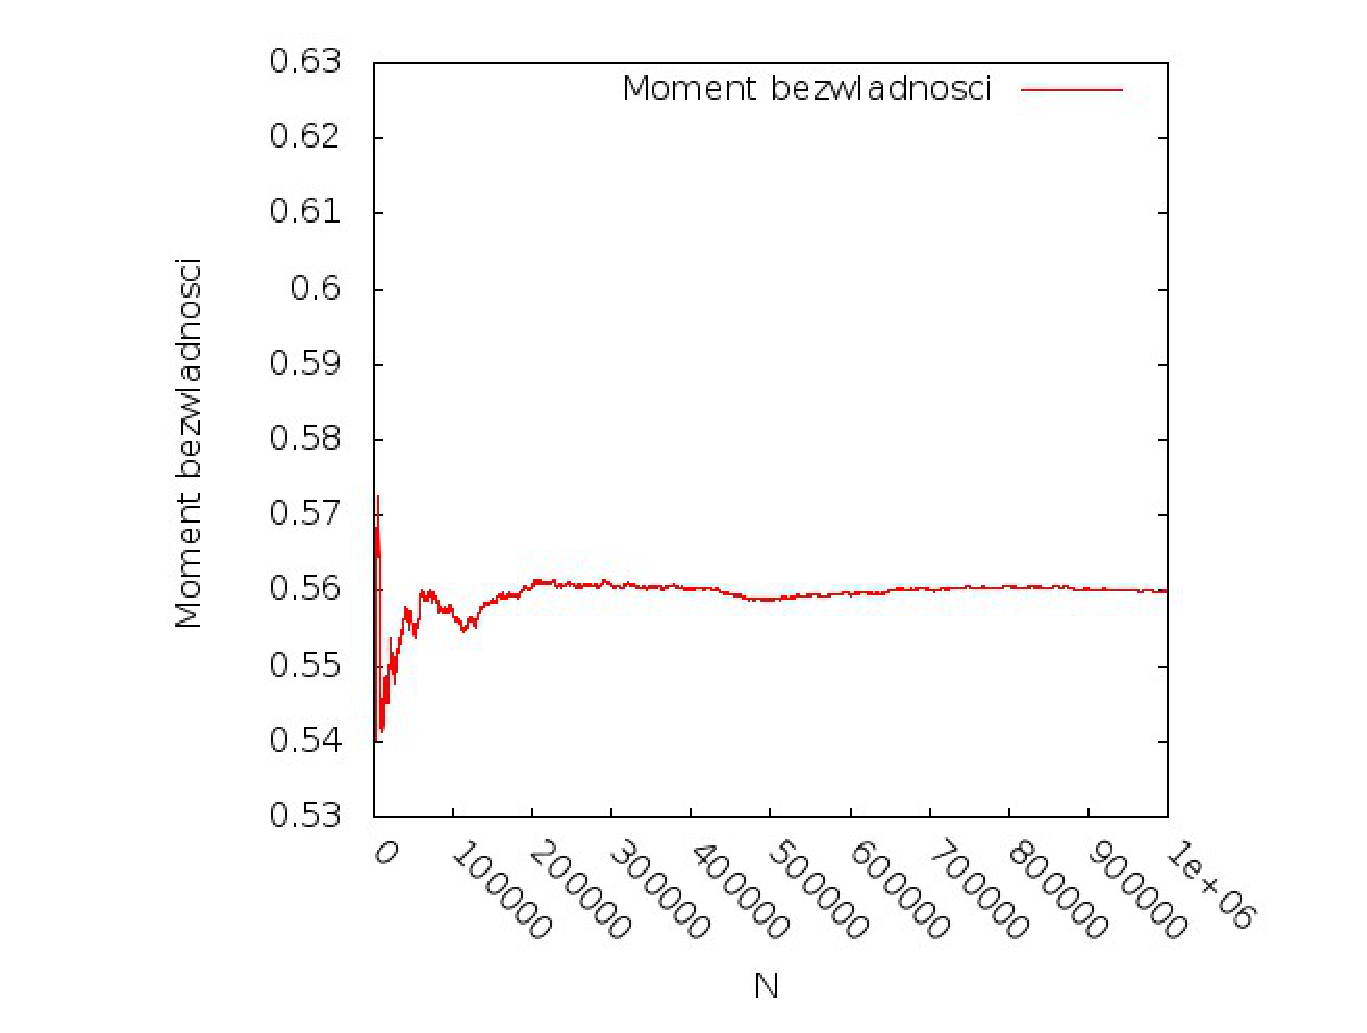
\includegraphics[scale=0.5]{plot.eps}
\end{figure}
\end{center}
\begin{figure}
\caption{Błąd oszacowania}
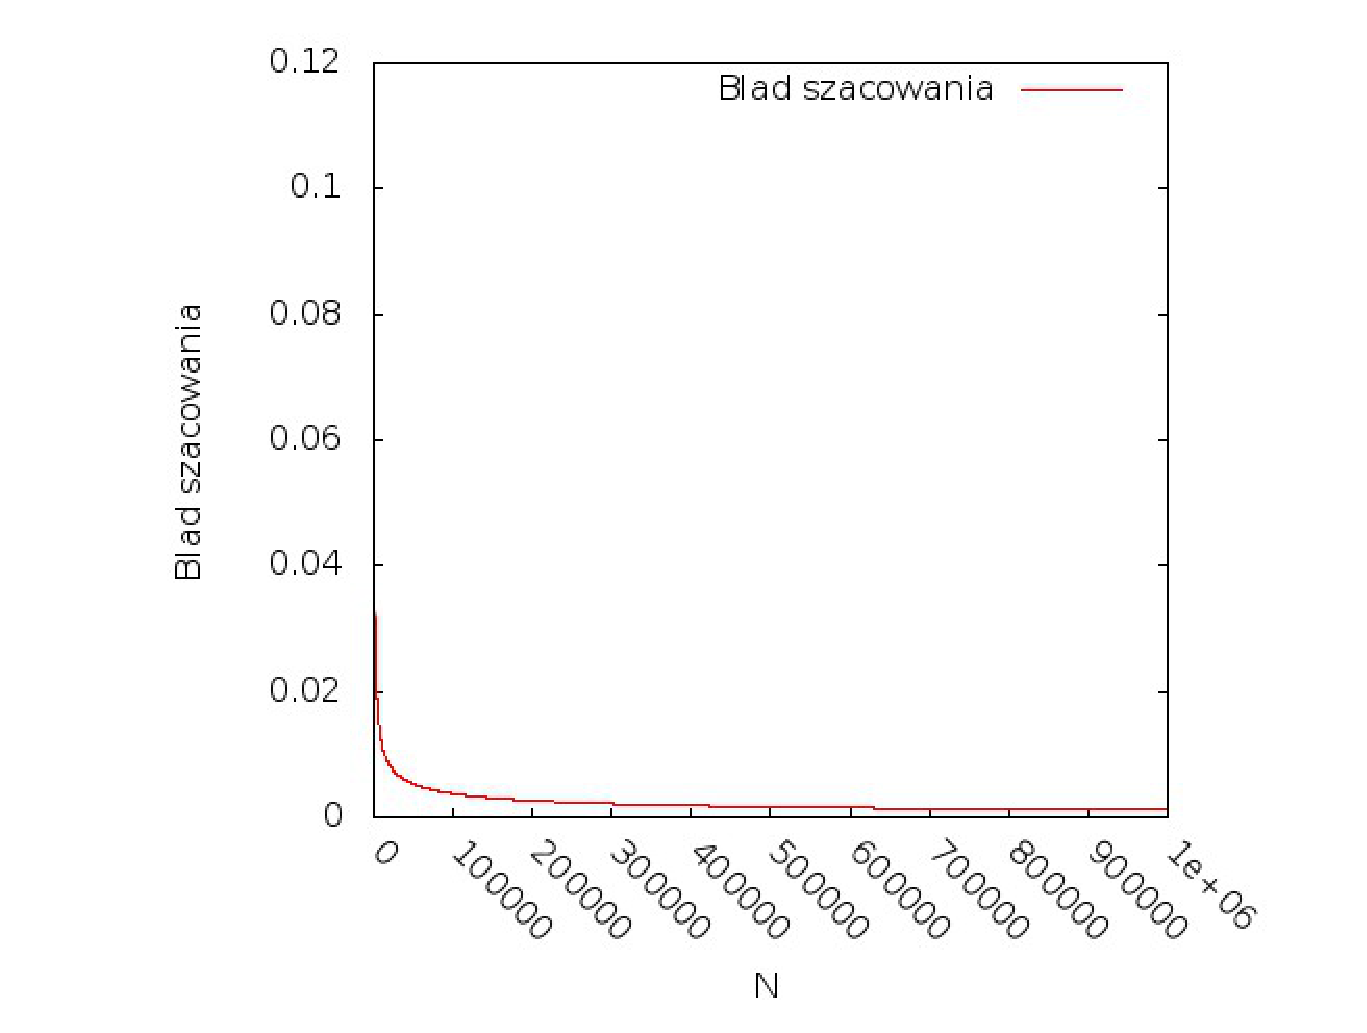
\includegraphics[scale=0.5]{plot2.eps}
\end{figure}
\item Wnioski\\
Powyższe wyniki otrzymywane są w~krótkim czasie a~dokładność ich jest zadowalająca w~stopniu inżynierskim. Oczekiwany moment bezwładności wyliczony ze wzoru dokładnego wynosi: $0,55794686$ natomiast otrzymamy metodą Monte Carlo wynosi: $0.560013$, co w~rozsądnym inżynierskim przybliżeniu jest wynikiem zadowalającym.\\
Powyższy przykład pokazuję zalety tej metody, łączące szybkość otrzymywanych wyników z~ich dokładnością.
\end{enumerate}
\end{document}
